Реально наблюдаемое в эксперименте число зеемановских линий существенным образом зависит от их относительных интенсивностей. Интенсивности зеемановских компонент могут быть рассчитаны из соображений симметрии. Результаты расчетов приведены в \ref{tab:1}.

В качестве примера приведем результаты расчета зеемановского спектра, соответствующего переходу 
$J\rightarrow J+1$
 между комбинирующими уровнями 
 $E_1(J_1=1,L_1=2,S_1=1)$ и $E_2(J_2=2,L_2=2,S_2=1)$,
  тогда согласно формуле \ref{eq:21} 
  $g_1=\frac12$, $g_2=\frac32$. 
  Переходы, на которых возможно получение зеемановских компонент, показаны стрелками на \ref{fig:3}, а в таблице \ref{tab:2} приведены поляризация и интенсивности соответствующих линий. 

% Как видно из \ref{eq:11} и таблиц \ref{tab:1}, \ref{tab:2}, зеемановский спектр зеркально симметричен относительно несмещенной линии, поэтому достаточно рассчитать половину спектра.
% ТАБЛИЦА 1
% РИСУНОК 3
% ТАБЛИЦА 2
\renewcommand{\arraystretch}{2}
\begin{table}[H]
    \caption{Относительные интенсивности зеемановских компонент}
    \label{tab:1}
    \centering
    %\resizebox{\textwidth}{!}{%
    \begin{tabular}{|c|c|c|c|c|}
     \hline
    \textbf{Переход} & $J\rightarrow J-1$ &$J\rightarrow J$ & $J\rightarrow J+1$ \\
    \hline
    \end{tabular}%
   % }
\end{table} 

\begin{table}[H]
    \setlength{\tabcolsep}{8pt}
    \caption*{Поперечный эффект}
    \centering 
    \begin{tabular}{|c|c|c|c|c|}
    \hline
    $M \rightarrow M-1$ & $ \frac{(J+M-1)(J+M)}{4} $ & $\frac{(J-M+1)(J+M)}{4}$ & $\frac{(J-M+2)(J-M+1)}{4}$ \\ \hline
    $M \rightarrow M$ & $ (J+M)(J-M) $ & $M^2$ & $(J+M+1)(J-M+1)$ \\ \hline
    $M \rightarrow M+1$ & $ \frac{(J-M-1)(J-M)}{4} $ & $\frac{(J+M+1)(J-M)}{4}$ & $\frac{(J+M+2)(J+M+1)}{4}$ \\ \hline
    \end{tabular}
\end{table}

\begin{table}[H]
    \setlength{\tabcolsep}{8pt}
    \caption*{Продольный эффект}
    \centering 
    \begin{tabular}{|c|c|c|c|c|}
    \hline
    $M \rightarrow M-1$ & $ \frac{(J+M-1)(J+M)}{2} $ & $\frac{(J-M+1)(J+M)}{2}$ & $\frac{(J-M+2)(J-M+1)}{2}$ \\ \hline
    $M \rightarrow M+1$ & $ \frac{(J-M-1)(J-M)}{2} $ & $\frac{(J+M+1)(J-M)}{2}$ & $\frac{(J+M+2)(J+M+1)}{2}$ \\ \hline
    \end{tabular}
\end{table}

\begin{figure}[H]
    \centering
    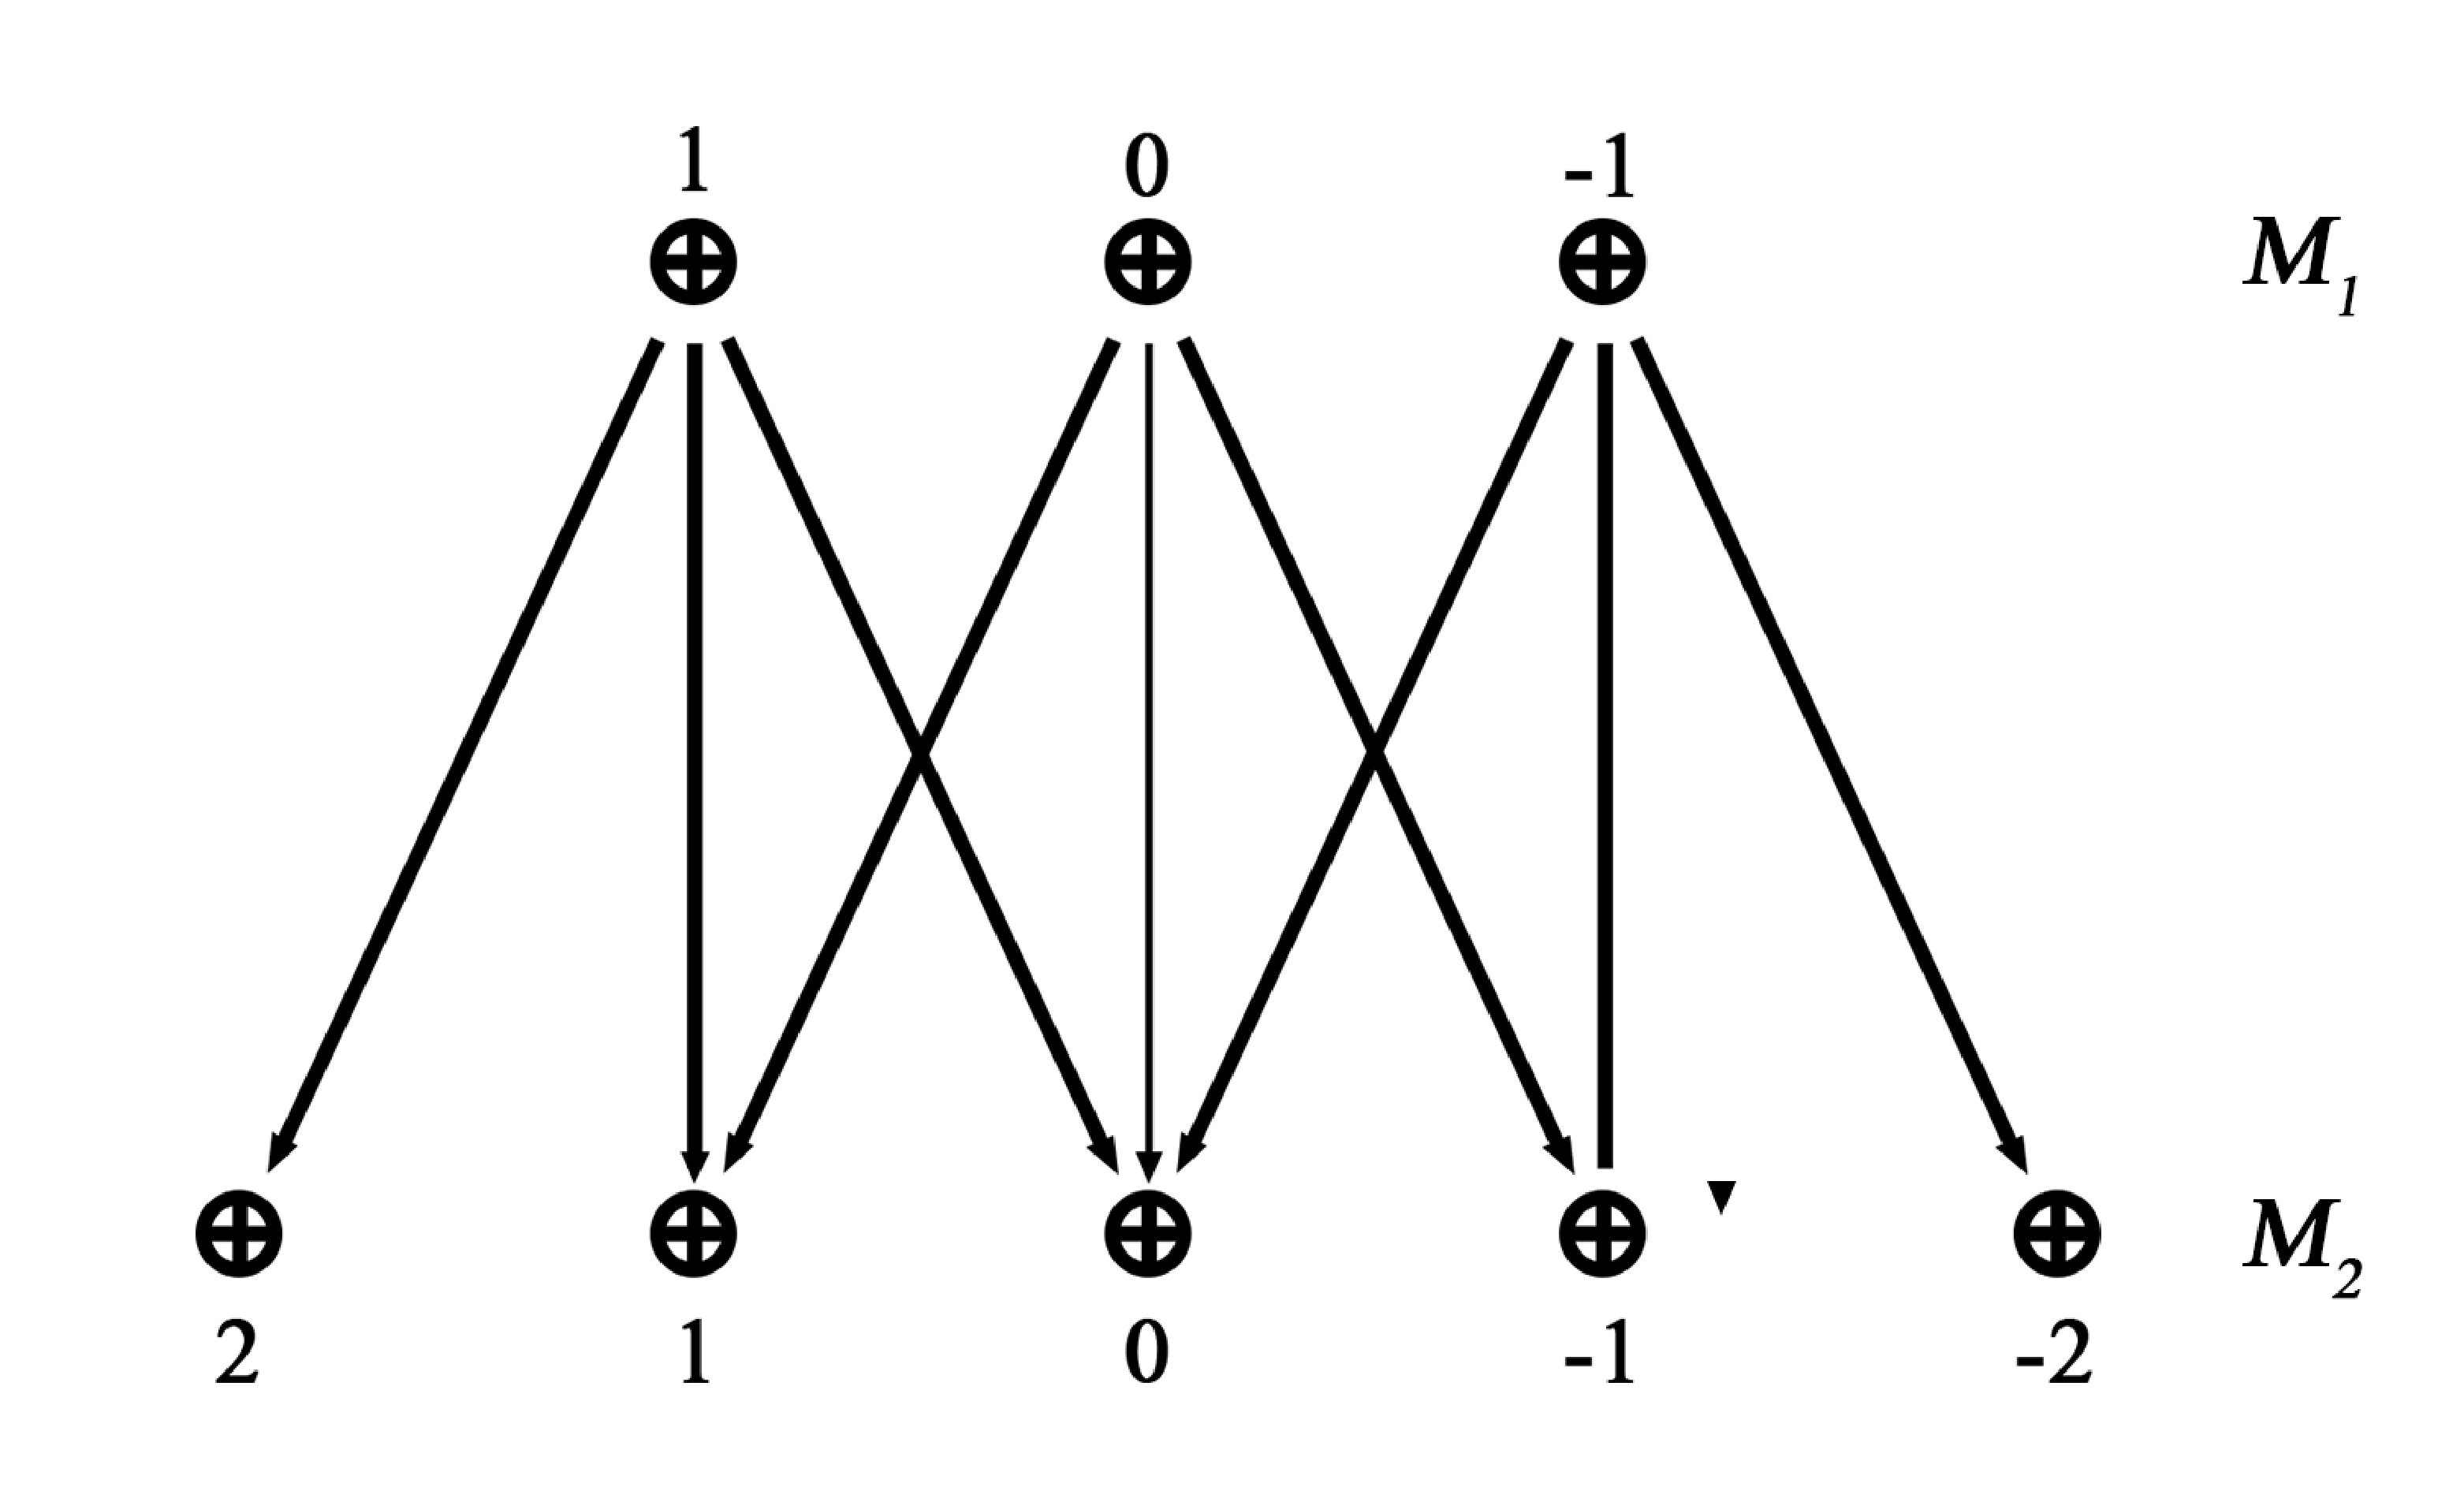
\includegraphics[width=.7\textwidth]{fig/fig3.pdf}
    \label{fig:3}
    \caption{Пример излучательных переходов, разрешенных правилами отбора}    
\end{figure}


\begin{table}[H]
    \setlength{\tabcolsep}{6pt}
    \caption{Поляризация и интенсивности линий Зеемановского спектра соответствующего переходу $J \rightarrow J+1$ между комбинирующими уровнями $ E_1(J_1=1,L_1=2,S_1=1)$ и $E_2(J_2=2,L_2=1,S_2=1) $} 
    \centering 
    \label{tab:2}
    \begin{tabular}{|p{8cm}|c|c|c|c|c|}
    \hline
    $\Delta \omega_{M_1 , M_2} * \hbar / (\mu_0 H) $ & \textbf{0} & $\mathbf{\pm 1/2}$ & $\mathbf{\pm 1}$ & $\mathbf{\pm 3/2}$ & $\mathbf{\pm 5/2}$ \\ \hline
    \textbf{Поляризация}  & $\mathbf{\boldsymbol\pi}$ & $ \mathbf{\boldsymbol\sigma} $ & $\mathbf{\boldsymbol\pi}$ & $ \mathbf{\boldsymbol\sigma} $ & $\mathbf{\boldsymbol\sigma} $ \\ \hline
    \textbf{Интенсивность}  (относительные единицы, поперечный эффект) & \textbf{4} &  \textbf{1/2} & \textbf{3}  &  \textbf{3/2} & \textbf{3} \\ \hline
    \end{tabular}
\end{table}
